\section{Détection de transcription}

\subsection{Les facteurs de transcription}
Le facteur de transcription est une proteine qui a pour but lire et transcrire l'ADN.\\
Pour cela, elle parcours le brin d'ADN jusqu'à trouver le site dont la forme des nucléotides lui correspond.

\subsection{JASPAR 2014}

JASPAR est la plus grande base de données en open source de nucleotides stoqué sous forme de matrice décrivant la liaison de facteurs de transcription sur plusieurs espèces.

\subsection{ChIP-Seq}

ChIP-Seq = Chromatin ImmunoPrecipitation Sequencing\\
C'est une méthode utilisée pour analyser les interactions entre les protéines et l’ADN.\\
Cette technologie combine l’immunoprécipitation de la chromatine (ChIP), en utilisant des anticorps spécifiques d’une protéine d’intérêt et le séquençage haut débit.\\
Le principe consiste à fixer de façon covalente les protéines liées à l’ADN par un traitement chimique, de fragmenter la chromatine, d’immunoprécipiter les fragments en présence de l’anticorps d’intérêt et après purification et élimination des protéines, de séquencer les fragments d’ADN obtenus.\\
Il est ainsi possible de cartographier tous les sites de liaison sur l’ADN de cette protéine à l’échelle du génome.

\subsection{Les Zingers}

Lorsque l'on utilise les ChIP-Seq pour transcrire un brin d'ADN, nous repérons plus facilement les motifs au milieu du bruit comme on le voit sur le motif Hnf4a ci-dessous.\\

\begin{figure}{l}{}
\centering
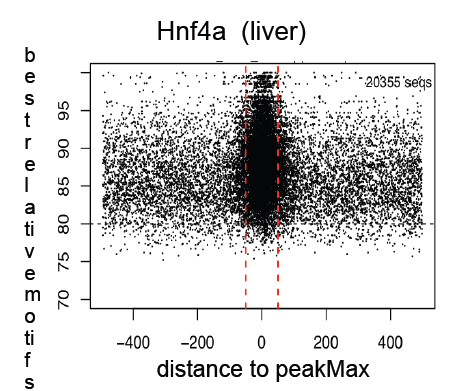
\includegraphics[scale=0.5]{peakmax}
\caption{Motif Hnf4a au milieu du bruit}
\end{figure}

Mais certain motifs apparaissent toujours peut importe la méthode utiliser sans que l'on comprennent réellement ce qu'il font là.\\
Ces motifs sont appelés ``Zingers''.
